% =============================================================================
% Chapter 9 — Performance Engineering: A First-Principles Account
% =============================================================================

\chapter{Performance Engineering: A First-Principles Account}
\label{ch:perf}

Adding a third node to this cluster cut the bytes each rank must stream per
decode step to $\approx$11.5\,GB, and the streaming model priced the step at
$\approx$48\,ms. Yet measured single-stream decode came out at 64.3
\tokspersec{} median, no faster than the August-published two-node band of
62--83. A hardware
change that provably reduced the dominant physical cost moved the end metric
by nothing: thirteen-plus milliseconds of fixed per-step cost ate the entire
bandwidth gain. That flat number is the cleanest measurement in the repository of
what a decode step's $\approx$108 collectives and fixed software overhead
actually cost. It frames the question this chapter answers: where does
the time in a decode step \emph{have} to go, and which knobs can still move
it?

\begin{figure}[htbp]
\centering
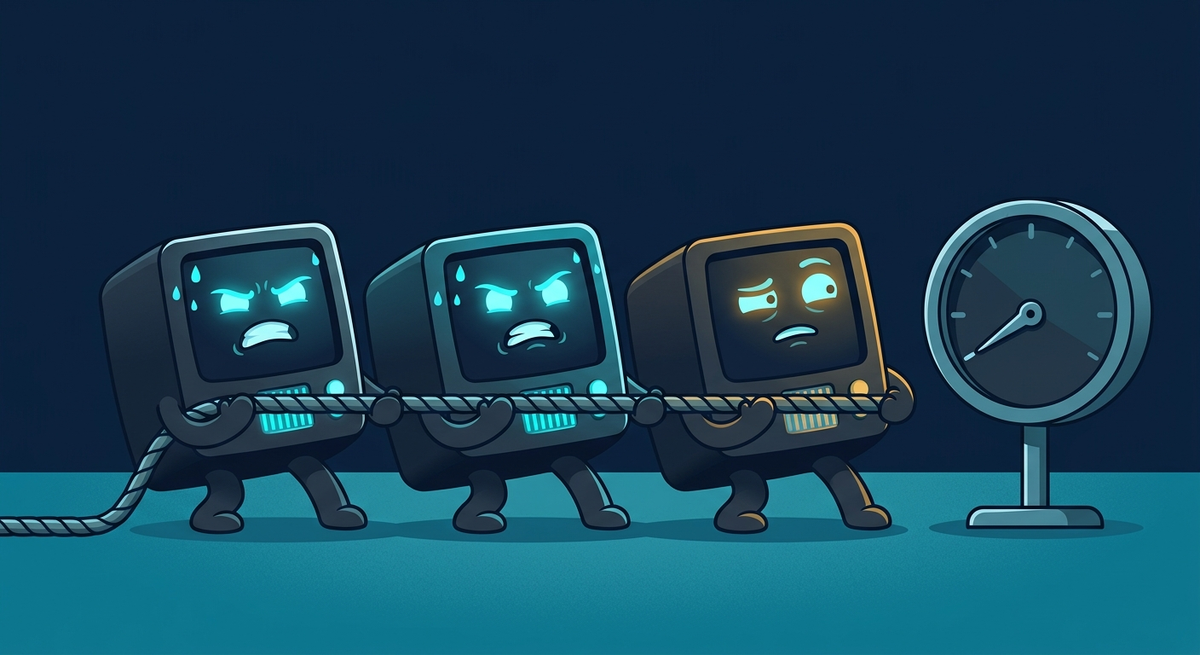
\includegraphics[width=0.80\textwidth]{figures/toon-ch09-thirdnode.png}
\caption{Everyone pulling harder; the needle unmoved. A third Spark provably cut the bytes each rank must stream per decode step to $\approx$11.5\,GB, and the streaming model priced the step at $\approx$48\,ms. Measured single-stream decode came out at 64.3 \tokspersec{} --- no faster than two nodes, because thirteen-plus milliseconds of fixed per-step cost ate the entire bandwidth gain. It is the cleanest measurement in either repository of what fixed overhead actually costs.}
\label{fig:toon-thirdnode}
\end{figure}

Every serving stack eventually accumulates a folklore of ``fast knobs'' --- flags
that someone once flipped before a good run. This repository refused to build
that folklore. Instead it built a cost model from the model's own weight shapes,
predicted where the time in a decode step must go, and then ran two disciplined
one-knob-per-boot A/B campaigns to test every prediction it could reach without
root or a kernel rebuild. The result is unusually honest: a handful of confirmed
wins, a longer list of confirmed \emph{non}-wins, one measured decline nobody
can yet explain, and a clear boundary line between what configuration can still
buy and what now requires engineering.

This chapter reconstructs that account for the inference engineer, because
the method --- model first, measure second, revert by default --- is the
transferable asset on any bandwidth-starved hardware. A cost model built from
weight shapes rules out entire classes of tuning before a single boot, and a
measurement protocol that knows its own noise floor is the only thing
standing between a verdict and an anecdote.

\section{The price of one decode step}
\label{sec:perf-costmodel}

The cost model is a subtraction. Price the bytes one step must move at the
memory bandwidth that actually exists, subtract that from the measured step
time, and whatever is left is fixed cost that no configuration knob reaches.

\subsection{Bytes per step: the streaming budget}

Start from what a single decode step at TP=2, $c=1$ must physically move. With
speculative decoding at $k=6$ (\Cref{ch:specdecode}), each step processes seven
query tokens --- one verified target token plus six draft tokens. The fable5-1
audit walked the checkpoint's shapes and produced a per-rank byte budget:

\begin{itemize}
  \item \textbf{Routed experts, $\approx$12\,GB.} Seven tokens each routing to
    top-6 of 256 experts per layer touch an expected $\approx$39 (at most 42)
    distinct experts, at 6.7\,MB per expert per rank, across 43 layers plus one
    shared expert (layers 0--2 hash-route by token id, so they pay the same
    streaming cost without a router GEMM).
  \item \textbf{Attention weights, $\approx$2.4\,GB.} The fp8 projections:
    the fused \code{fused_wqa_wkv} path, the replicated indexer projections
    (\code{wq_b}, \code{weights_proj}), and the sharded \code{wq_b},
    \code{wo_a}, \code{wo_b}.
  \item \textbf{Draft model, $\approx$0.9\,GB.} Three DSV4 MTP layers over six
    query tokens, touching $\approx$36 expert slots.
  \item \textbf{\code{lm_head}, $\approx$1.06\,GB.} The bf16
    $129{,}280 \times 4{,}096$ sharded head, read for both target and draft
    base logits.
  \item \textbf{Markov head, $\approx$0.2\,GB.} The draft's Markov \code{w2}
    read six times (33\,MB per rank per read).
\end{itemize}

The total, $\approx$16.5--17\,GB per rank per step, is the number the whole
chapter hangs on. At the DGX Spark's effective LPDDR5X bandwidth of
230--250\,GB/s that is 68--74\,ms of unavoidable weight streaming per step
(\Cref{fig:perf-bytebudget}). With $\approx$4.15 accepted tokens per step, the
streaming bound alone predicts 56--61 \tokspersec{}, against the
August-published $c=1$ band of
62--83 \tokspersec{}. The conclusion the audit drew: \textbf{roughly 80\,\% of a
$c=1$ decode step is weight streaming}, and the residual $\approx$10--15\,ms is
fixed per-step cost. No configuration knob doubles $c=1$, because no
configuration knob changes how many bytes an expert weighs.

\begin{figure}[htbp]
\centering
\adjustbox{max width=\textwidth}{%
\begin{tikzpicture}[font=\small]
  % scale: 0.72 cm per GB; segments: 12 / 2.4 / 1.06 / 0.9 / 0.2 GB
  \def\perfbh{1.0} % bar height
  % experts
  \fill[hbBlue!25]  (0,0)      rectangle (8.64,\perfbh);
  \fill[hbGreen!30] (8.64,0)   rectangle (10.37,\perfbh);
  \fill[hbAmber!35] (10.37,0)  rectangle (11.13,\perfbh);
  \fill[hbSteel!30] (11.13,0)  rectangle (11.78,\perfbh);
  \fill[hbAccent!30](11.78,0)  rectangle (11.92,\perfbh);
  \draw[hbSteel,thick] (0,0) rectangle (11.92,\perfbh);
  \draw[hbSteel!60] (8.64,0) -- (8.64,\perfbh);
  \draw[hbSteel!60] (10.37,0) -- (10.37,\perfbh);
  \draw[hbSteel!60] (11.13,0) -- (11.13,\perfbh);
  \draw[hbSteel!60] (11.78,0) -- (11.78,\perfbh);
  % in-bar labels for the big segments
  \node at (4.32,0.5)  {routed experts $\approx$12\,GB};
  \node[font=\scriptsize] at (9.5,0.5) {attn $\approx$2.4};
  % leader labels for the small segments
  \node[hblabel,anchor=west] (lh) at (12.15,-0.35) {lm\_head $\approx$1.06\,GB};
  \draw[hbSteel!70] (10.75,0) -- (12.1,-0.35);
  \node[hblabel,anchor=west] (dr) at (12.15,-0.95) {draft $\approx$0.9\,GB};
  \draw[hbSteel!70] (11.45,0) -- (12.1,-0.95);
  \node[hblabel,anchor=west] (mk) at (12.15,-1.55) {Markov w2 $\approx$0.2\,GB};
  \draw[hbSteel!70] (11.85,0) -- (12.1,-1.55);
  % total annotation
  \draw[decorate,decoration={brace,amplitude=5pt},hbBlue,thick]
    (0,\perfbh+0.15) -- (11.92,\perfbh+0.15);
  \node[hbtitle,anchor=south] at (5.96,\perfbh+0.42)
    {$\approx$16.5--17\,GB/rank/step $\;\rightarrow\;$ 68--74\,ms at 230--250\,GB/s effective};
  \node[hblabel,anchor=north west] at (0,-2.35)
    {TP=2, $c=1$, $k=6$: 7 query tokens/step (1 target + 6 draft); measured step implies
     $\approx$80\,\% streaming + 10--15\,ms fixed cost.};
\end{tikzpicture}%
}
\caption{The decode-step byte budget at TP=2, $c=1$. Expert streaming dominates:
seven query tokens route to $\approx$39 distinct experts per layer across 43
layers. At effective memory bandwidth this budget alone predicts 56--61 \tokspersec{}
at $\approx$4.15 accepted tokens/step, against the August-published
62--83 \tokspersec{} band ---
decode is $\approx$80\,\% weight-streaming-bound.}
\label{fig:perf-bytebudget}
\end{figure}

\subsection{The collectives census: $\approx$108 per step}

The fixed cost is not mysterious; the audit counted it. One TP=2 decode step
issues approximately 108 NCCL collectives (\Cref{fig:perf-collectives}):

\begin{itemize}
  \item 43 \code{wo_b} all-reduces (one per layer's output projection),
  \item 43 MoE all-reduces,
  \item 6 draft-layer all-reduces,
  \item 2 embedding all-reduces,
  \item 2 logits all-gathers --- \code{use_all_gather()} is true on CUDA, so
    every rank gathers \emph{full} logits (10.9\,MB at $c=6$),
  \item 12 serialized collectives in the Markov draft loop.
\end{itemize}

\begin{sloppypar}
The last item deserves its own sentence. The DSpark Markov head is TP-sharded
(\code{VocabParallelEmbedding} plus \code{ParallelLMHead}), and the draft
sampler runs six \emph{dependent} iterations of embed--bias--sample. Each
iteration carries one all-reduce and one all-gather of a
$[\text{num\_reqs} \times 129{,}280]$ logits tensor. The kernels live inside the
draft's CUDA graph, so there is no launch overhead --- but the network
round-trips serialize, twelve in a row, every step. At 30--50\,$\mu$s
per collective on RoCE (no GPUDirect on GB10 --- every collective bounces
through a host buffer), the census totals $\approx$3--5\,ms per step: 5--8\,\%
of a $c=1$ step, 2--3\,\% at $c=6$.
\end{sloppypar}

\begin{figure}[htbp]
\centering
\adjustbox{max width=\textwidth}{%
\begin{tikzpicture}[font=\small]
  % scale: 0.11 cm per collective; 43 + 43 + 6 + 2 + 2 + 12 = 108
  \def\colb{1.0}
  \fill[navy!30]      (0,0)     rectangle (4.73,\colb);
  \fill[navy!15]      (4.73,0)  rectangle (9.46,\colb);
  \fill[teal!32]      (9.46,0)  rectangle (10.12,\colb);
  \fill[teal!22]      (10.12,0) rectangle (10.34,\colb);
  \fill[teal!12]      (10.34,0) rectangle (10.56,\colb);
  \fill[brandcyan!45] (10.56,0) rectangle (11.88,\colb);
  \draw[brandgray,thick] (0,0) rectangle (11.88,\colb);
  \foreach \x in {4.73,9.46,10.12,10.34,10.56} {
    \draw[brandgray!60] (\x,0) -- (\x,\colb);
  }
  \draw[brandcyan!70!black,very thick] (10.56,0) rectangle (11.88,\colb);
  % in-bar labels for the two 43-wide segments
  \node[align=center] at (2.365,0.5) {\textbf{43}\\\texttt{wo\_b} all-reduces};
  \node[align=center] at (7.095,0.5) {\textbf{43}\\MoE all-reduces};
  % total
  \node[hbtitle,anchor=south west] at (0,1.15)
    {$\approx$108 collectives per TP=2 decode step};
  % fan of leader labels for the narrow segments
  \node[hblabel,anchor=west] at (12.15,3.20) {\textbf{6} draft-layer all-reduces};
  \draw[brandgray!70] (9.79,\colb) -- (12.10,3.20);
  \node[hblabel,anchor=west] at (12.15,2.55) {\textbf{2} embedding all-reduces};
  \draw[brandgray!70] (10.23,\colb) -- (12.10,2.55);
  \node[hblabel,anchor=west] at (12.15,1.90) {\textbf{2} logits all-gathers};
  \draw[brandgray!70] (10.45,\colb) -- (12.10,1.90);
  \node[hblabel,anchor=west,color=brandcyan!70!black] at (12.15,1.25)
    {\textbf{12} Markov loop};
  \draw[brandcyan!70!black] (11.22,\colb) -- (12.10,1.25);
  \node[hbfaint,anchor=north west,align=left,font=\scriptsize,text width=41mm]
    at (12.15,0.95)
    {\texttt{use\_all\_gather()} true on CUDA --- full logits, 10.9\,MB at $c=6$\\[2pt]
     \texttt{VocabParallelEmbedding} / \texttt{ParallelLMHead}};
  % pull the serialized dozen down into a sequence strip
  \draw[brandcyan!70!black,dashed] (10.56,0) -- (0,-1.45);
  % right leader dropped down the near side of the note box, then across below it
  \draw[brandcyan!70!black,dashed] (11.88,0) -- (12.00,-1.05) -- (16.20,-1.45);
  % cells sized to the label they hold, with clear space on both sides
  \foreach \i in {0,1,2,3,4,5} {
    \fill[ice] ({\i*2.70},-2.25) rectangle ({\i*2.70+2.70},-1.45);
    \draw[brandgray!45] ({\i*2.70+0.90},-2.25) -- ({\i*2.70+0.90},-1.45);
    \draw[brandgray!45] ({\i*2.70+1.62},-2.25) -- ({\i*2.70+1.62},-1.45);
    \draw[brandcyan!70!black,thick] ({\i*2.70},-2.25) rectangle ({\i*2.70+2.70},-1.45);
    \node[font=\tiny,anchor=base] at ({\i*2.70+0.45},-1.90) {embed};
    \node[font=\tiny,anchor=base] at ({\i*2.70+1.26},-1.90) {bias};
    \node[font=\tiny,anchor=base] at ({\i*2.70+2.16},-1.90) {sample};
  }
  \node[hblabel,anchor=north] at (8.1,-2.40)
    {each of six dependent iterations: 1 all-reduce $+$ 1 all-gather
     $[\text{num\_reqs} \times 129{,}280]$};
  \node[hbpatch,anchor=north,align=center,font=\scriptsize,text width=126mm]
    at (8.1,-2.90)
    {serialized --- each position's Markov bias depends on the token chosen
     at the previous one};
  \node[hblabel,anchor=north] at (8.1,-3.95)
    {kernels live inside the draft's CUDA graph --- no launch overhead;
     the network round-trips serialize};
  % pricing footer
  \draw[brandgray!50] (0,-4.65) -- (16.35,-4.65);
  \node[hblabel,anchor=north west] at (0,-4.85)
    {30--50\,$\mu$s per collective on RoCE};
  \draw[brandgray!40] (4.60,-4.75) -- (4.60,-5.20);
  \node[hblabel,anchor=north west] at (4.80,-4.85) {no GPUDirect on GB10};
  \draw[brandgray!40] (8.30,-4.75) -- (8.30,-5.20);
  \node[hblabel,anchor=north west] at (8.50,-4.85)
    {$\approx$3--5\,ms per step $=$ 5--8\,\% of a $c=1$ step, 2--3\,\% at $c=6$};
  % closing row: cost-model chip and the TP=3 annotation
  \node[hbbox,anchor=north west,align=left,font=\scriptsize,text width=64mm]
    at (0,-5.40)
    {bytes (68--74\,ms) $+$ fixed cost (10--15\,ms) $=$ the step};
  \node[hbpatch,anchor=north west,align=left,font=\scriptsize,text width=74mm]
    at (8.50,-5.40)
    {\textbf{TP=3: $\approx$11.5\,GB/rank, $\approx$48\,ms predicted,
     64.3 \tokspersec{} measured}\\[2pt]
     three-rank ring $\approx2\times$ the latency; heads padded $64 \to 72$;
     ring spans two physical links};
\end{tikzpicture}%
}
\caption{The other half of the cost model. One TP=2 decode step issues
approximately 108 NCCL collectives --- 43 \code{wo_b} all-reduces, 43 MoE
all-reduces, 6 draft-layer all-reduces, 2 embedding all-reduces, 2
full-logits all-gathers (10.9\,MB at $c=6$, since \code{use_all_gather()} is
true on CUDA), and the 12 in the Markov draft loop. At 30--50\,$\mu$s per
collective on RoCE --- with no GPUDirect on GB10, so every collective bounces
through a host buffer --- that is roughly 3--5\,ms per step, 5--8\,\% of a
$c=1$ step. The Markov dozen are the only entries that cannot overlap: six
dependent iterations of embed--bias--sample, each carrying one all-reduce and
one all-gather, serialized because each position's bias depends on the
previous token. This fixed cost is what made TP=3's drop to $\approx$11.5\,GB
per rank --- priced at $\approx$48\,ms --- arrive as 64.3 \tokspersec{}, no
faster than two nodes.}
\label{fig:perf-collectives}
\end{figure}

\subsection{The TP=3 natural experiment}

The strongest evidence that fixed cost, not bandwidth, now governs $c=1$
came free of charge --- it is the flat TP=3 result the chapter opened with.
At audit time the cluster happened to be running the three-node TP=3
experiment (\Cref{ch:scaling}). The mechanism behind the flat number is
exactly the fixed cost this section has been counting: a three-rank ring has
roughly twice the latency of a two-rank exchange, the attention heads are
padded $64 \to 72$ to divide by three, and the ring spans two different
physical links. As the opening showed, that fixed cost ate the entire
bandwidth gain the streaming model had priced in. TP=3 is a capacity win
(5.0\,M KV tokens, 16 slots, $4.79\times$ concurrency at 1M) --- it is not a
latency win, and the cost model says it cannot be until the fixed per-step
costs shrink.

\begin{hblesson}
When a hardware upgrade that provably reduces the dominant physical cost
(bytes per rank) fails to move the end metric, you have measured your fixed
overhead more convincingly than any profiler would. The TP=3 boot was run for
capacity; its flat $c=1$ number is the cleanest single measurement in the repository
of what the $\approx$108 collectives and eager launches cost.
\end{hblesson}

\section{Where throughput actually comes from}
\label{sec:perf-throughput}

The decode side has exactly two multipliers, and both work the same way:
spreading one weight stream over more tokens. Concurrency supplies those
tokens from other requests, speculative acceptance from the same one.
Prefill, as the last part of this section shows, obeys different economics
entirely.

\subsection{Concurrency amortizes the weight stream}

If one step must stream 16.5\,GB regardless, the obvious move is to make each
step serve more tokens. The same expert weights read once serve every sequence
in the batch, so aggregate throughput climbs steeply with concurrency while
per-stream rates fall gently. The published 1~August sweep at 256-token prompts
shows the curve exactly (\Cref{fig:perf-concurrency}): aggregate 69.1 \tokspersec{} at
$c=1$, 104.9 at $c=2$, 164.5 at $c=4$, 191.2 at $c=6$ --- while per-stream
decode declines 75.4 $\to$ 58.3 $\to$ 46.8 $\to$ 36.9 \tokspersec{}. Six concurrent
chats buy roughly $2.8\times$ the fleet throughput of one on that sweep (the
audit quotes $\approx$$2.2\times$ against its own published TP=2 reference
band), because the marginal sequences ride a weight stream that was being paid
for anyway.

\begin{figure}[htbp]
\centering
\begin{tikzpicture}[font=\small]
  % x: concurrency 0..6.8 at 1.5cm/unit ; y: tok/s 0..200 at 0.026 cm per tok/s
  \def\perfX#1{#1*1.5}
  \def\perfY#1{#1*0.026}
  % grid
  \foreach \y in {50,100,150,200} {
    \draw[hbSteel!25] (0,\perfY{\y}) -- (\perfX{6.8},\perfY{\y});
    \node[hblabel,anchor=east] at (-0.1,\perfY{\y}) {\y};
  }
  \draw[hbarrow] (0,0) -- (\perfX{7.1},0) node[hblabel,anchor=north west,yshift=-1mm] {concurrency $c$};
  \draw[hbarrow] (0,0) -- (0,\perfY{210}) node[hblabel,anchor=south] {\tokspersec{}};
  \foreach \c in {1,2,4,6} {
    \draw[hbSteel] (\perfX{\c},0) -- (\perfX{\c},-0.08);
    \node[hblabel,anchor=north] at (\perfX{\c},-0.1) {\c};
  }
  % aggregate line
  \draw[hbflow,very thick]
    (\perfX{1},\perfY{69.1}) -- (\perfX{2},\perfY{104.9}) -- (\perfX{4},\perfY{164.5}) -- (\perfX{6},\perfY{191.2});
  \foreach \c/\v in {1/69.1,2/104.9,4/164.5,6/191.2} {
    \fill[hbBlue] (\perfX{\c},\perfY{\v}) circle (2pt);
    \node[hblabel,color=hbBlue,anchor=north west] at (\perfX{\c}+0.08,\perfY{\v}-0.06) {\v};
  }
  \node[hbtitle,anchor=west] at (\perfX{4.35},\perfY{188}) {aggregate};
  % per-stream line
  \draw[color=brandgreen!70!black,very thick,dashed]
    (\perfX{1},\perfY{75.4}) -- (\perfX{2},\perfY{58.3}) -- (\perfX{4},\perfY{46.8}) -- (\perfX{6},\perfY{36.9});
  \foreach \c/\v in {1/75.4,2/58.3,4/46.8,6/36.9} {
    \fill[hbGreen!70!black] (\perfX{\c},\perfY{\v}) circle (2pt);
  }
  \node[hblabel,color=hbGreen!60!black,anchor=north west] at (\perfX{4.15},\perfY{31}) {per-stream};
\end{tikzpicture}
\caption{Aggregate and per-stream decode \tokspersec{} versus concurrency, 256-token
prompts, natural completions (published 1~August 2026 sweep). Aggregate climbs
$69.1 \to 191.2$ \tokspersec{} from $c=1$ to $c=6$ --- roughly $2.8\times$ on this
sweep, against the audit's $\approx$$2.2\times$ rule of thumb for the published
TP=2 band --- because concurrent sequences amortize the same 16.5\,GB/step
weight stream; per-stream rates decline gently from 75.4 to 36.9 \tokspersec{}.}
\label{fig:perf-concurrency}
\end{figure}

\subsection{Acceptance is the other multiplier}

The second throughput lever divides rather than multiplies: bytes per
\emph{accepted} token, since every accepted draft token is a token generated
without another 16.5\,GB step. Acceptance is strongly prompt-dependent on
this draft head --- roughly half the drafted tokens accepted on
numbered-word probes versus a quarter on live natural prose --- and that gap,
not any \repofile{.env} knob, is the largest remaining decode lever
(\Cref{sec:perf-remains}). The mechanism, the curves, and the probe
discipline are \Cref{ch:specdecode}'s subject.

\subsection{Prefill obeys different economics}

Decode is bandwidth-bound; prefill is compute- and kernel-bound, and at long
context one component dominates everything: the Lightning indexer. The indexer
is \emph{replicated} across TP ranks (\code{wq_b} and \code{weights_proj} are
\code{ReplicatedLinear} --- the source comments ``no tensor parallel, just
replicated''), so every rank scores all 64 index heads against the entire
compressed key range. The work is $O(\text{queries} \times \text{keys})$: at
900K context each 1{,}024-token chunk costs $\approx$80\,TFLOP of scoring,
$\approx$0.8\,s of tensor-core time, \emph{duplicated on both GPUs}. That
quadratic term is why prefill falls from 2{,}563 \tokspersec{} at 2K context to
$\approx$875 \tokspersec{} on the 900K acceptance run (899{,}994 prompt tokens,
1{,}028.85\,s TTFT).

The MoE path compounds it at short and medium context:
b12x runs W4A16 (dequantize to bf16) for the checkpoint's
\code{fp4_e8m0_k32} expert format because its NVFP4 tensor-core path accepts
only modelopt-format weights. The largest prefill FLOP consumer therefore
runs at roughly a quarter of the hardware's FP4$\times$FP8 rate. Streaming,
collectives, replicated indexer scoring, dequantized MoE: each of these
costs is attackable at a very different price, and ranking those prices is
what the audit did next.

\section{Ten findings, ranked by expected value over effort}
\label{sec:perf-findings}

The audit distilled everything above into ten ranked findings
(\Cref{tab:perf-findings}). The ranking discipline matters as much as the
content: each row states a mechanism, an evidence trail, an \emph{expected}
effect with an honest error bar, and the effort class --- host command, one
compose line, a $\sim$60-line patch, or multi-day kernel work. Findings are
predictions until measured; \Cref{sec:perf-ab} is where several of them met
reality.

\begin{table}[htbp]
\centering
\small
\caption{The fable5-1 audit's ten findings, ranked by expected value over
effort (condensed from the 2026-09-02 report).}
\label{tab:perf-findings}
\begin{tabular}{@{}cl>{\raggedright\arraybackslash}p{5.2cm}>{\raggedright\arraybackslash}p{3.4cm}>{\raggedright\arraybackslash}p{2.5cm}@{}}
\toprule
\# & Class & Finding & Expected effect & Effort \\
\midrule
1 & stability & Host memory exhausted at boot on both nodes (\code{NV_ERR_NO_MEMORY}; worker swap 10.4\,GB, polkitd leak 3.1\,GB; KV pool sized from the worst rank) & reclaim 5--8\,GB $\to$ util $0.83 \to 0.86$--$0.88$ = +20--35\,\% KV tokens & host-side + restart \\
2 & config & $c=6$ decode shape (42 tokens) not CUDA-graph captured: argv 42 truncated to 40, rounded to multiples of 7 $\to$ graphs [7,14,21,28,35]; $c=6$ runs eager & +3--10\,\% $c=6$ aggregate & one compose line \\
3 & fabric & NCCL pinned to one CX7 PCIe function (Gen5 $\times$4 $\approx$ 126\,Gb/s feeding a 200\,Gb/s port); RoCE MTU 1024; duplicate subnet on the second PF & prefill comm up to $\sim$2$\times$; decode unchanged & host + env \\
4 & patch & Markov head TP-sharded $\to$ 12 serialized collectives/step; both matrices 66\,MB, replication free & $-$12 collectives $\approx$ 0.5--1.5\,ms (1--3\,\%) & $\sim$60-line patch \\
5 & kernel & W4A16 everywhere: no MXFP4 tensor-core MoE for \code{fp4_e8m0_k32}; \envvar{B12X_W4A16_TC_DECODE} untested and not plumbed through compose & TC-decode 0--10\,\% $c=1$ (A/B); MXFP4 MoE $\to$ prefill +30--60\,\% & env now; kernels later \\
6 & engineering & Lightning indexer replicated across ranks; dominates prefill at $\geq$128K & sequence-parallel indexer $\to$ up to $\sim$1.8$\times$ long-context prefill & multi-day \\
7 & patch & Static 1024-token prefill chunk cap even with no decode lanes active & $c=1$ TTFT $-$10--25\,\% on $\leq$32K prompts & $\sim$30-line patch \\
8 & upstream & \code{nvfp4_ds_mla} is byte-identical to \code{fp8_ds_mla} (584\,B/row) --- no 4-bit KV today & true NVFP4 row $\to$ +50\,\% KV tokens & FlashInfer SM120 work \\
9 & fairness & Live \envvar{DSPARK_MAX_INFLIGHT_PREFILLS}=2 despite the \ghissue{154} revert to 1 & decide explicitly (fairness vs the 32K$\times$c4 floor) & \repofile{.env} + restart \\
10 & latency & Warmup gaps: sparse-MLA autotune covers only tokens=16; CuTeDSL warmup skipped; first requests JIT mid-serve & removes first-request cliffs; closes the JIT-vs-watchdog hazard (\ghissue{117}) & scripts + restart \\
\bottomrule
\end{tabular}
\end{table}

Finding \#1, the top-ranked row, deserves a trace of its own, because its
punchline is structural. During the audited boot, both nodes' kernel logs
recorded repeated \code{NVRM: Out of memory [NV_ERR_NO_MEMORY]} allocation
failures in the profile/autotune/capture window --- the boot survived only
because the failing allocations were retried elsewhere. The worker was the
worse host: 5.4\,GB MemAvailable, 10.4\,GB of swap in use, and a
\code{polkitd} process holding 3.1\,GB of RSS (a known polkit leak under
GNOME). The node was still on \code{graphical.target}, with Xorg and
gnome-shell holding GPU contexts.

The consequence reaches past one machine:
the worker's KV pool came out 1.19\,GiB below the head's (33.82 versus
35.01\,GiB), and vLLM sizes the shared pool from the \emph{worst} rank.
One leaky daemon on one node thus taxed the whole cluster's KV capacity. That
chain --- host bloat, worst-rank sizing, fleet-wide KV loss --- is what
drives the host-memory gate of \Cref{sec:perf-ab}, the unified-memory
warning below it, and the root-only hunt of \Cref{sec:perf-remains}.

Finding \#2 is worth tracing in full because it became the book's cleanest
predict--fix--verify arc. The compose file computes the CUDA-graph capture size
as \code{MAX_NUM_SEQS} $\times$ (\code{MTP_NUM_TOKENS}$+1$) $= 42$. vLLM's
default capture list is $[1,2,4,8,16,24,32,40]$, and 42 is not on the stride.
The boot log therefore prints, verbatim, \code{Truncating max_cudagraph_capture_size to
40}, and spec-decode rounding then yields FULL graphs at $[7,14,21,28,35]$
only. A six-request decode step is exactly 42 tokens --- it dispatches to
\emph{no} graph and runs fully eager, issuing 1{,}500--1{,}800 Python-launched
kernels (\Cref{fig:perf-captureladder}).

\begin{hbnote}
The trace also exhumed a perfect measurement parable. An earlier
(19~August) A/B had concluded ``no $c=6$ lift'' --- but it ran at $k=5$ with
a capture cap of 32, whose $c=6$ shape (36 tokens) was \emph{also}
uncaptured in both arms. Both arms ran the untested configuration; the
experiment never tested the question. Gates before numbers exist precisely
because a clean-looking A/B can be null by construction.
\end{hbnote}

The fix is one line of compose arithmetic:

\begin{lstlisting}[language=bash]
# docker-compose.dspark.yml: round the capture size up to a multiple of 8
--max-cudagraph-capture-size $(( (MAX_NUM_SEQS*(MTP_NUM_TOKENS+1)+7)/8*8 ))
# 6*(6+1)=42 -> 48; boot gate: no "Truncating", "Capturing CUDA graphs (FULL) 6/6"
\end{lstlisting}

\begin{figure}[htbp]
\centering
\adjustbox{max width=\textwidth}{%
\begin{tikzpicture}[font=\small]
  % one shared token-count scale: x = 3.0 + 0.2*tokens, 0..48
  % ---------- row 1: vLLM's default capture list ----------
  \node[anchor=east,align=right,font=\scriptsize,text width=33mm] at (2.70,0)
    {\textbf{vLLM default capture list}\\\texttt{[1,2,4,8,16,24,32,40]}};
  \draw[navy,thick] (3.0,0) -- (12.6,0);
  \foreach \t in {1,2,4,8,16,24,32,40} {
    \draw[navy] ({3.0+0.2*\t},0) -- ({3.0+0.2*\t},-0.12);
    \node[font=\tiny,anchor=north,color=navy] at ({3.0+0.2*\t},-0.14) {\t};
  }
  \draw[clueerror,thick] (11.28,-0.12) -- (11.52,0.12);
  \draw[clueerror,thick] (11.28,0.12)  -- (11.52,-0.12);
  \node[hblabel,color=clueerror,anchor=south east] at (11.20,0.10)
    {42 is not on the stride};
  % ---------- row 2: after truncation ----------
  \node[anchor=east,align=right,font=\scriptsize,text width=33mm] at (2.70,-2.0)
    {\textbf{after truncation}\\\texttt{[7,14,21,28,35] FULL}};
  \node[anchor=west,font=\scriptsize\ttfamily,color=clueerror] at (3.0,-1.42)
    {Truncating max\_cudagraph\_capture\_size to 40};
  \fill[amber!25] (10.0,-2.25) rectangle (11.4,-1.75);
  \draw[navy,thick] (3.0,-2.0) -- (12.6,-2.0);
  \foreach \t in {7,14,21,28,35} {
    \draw[navy] ({3.0+0.2*\t},-2.0) -- ({3.0+0.2*\t},-2.12);
    \node[font=\tiny,anchor=north,color=navy] at ({3.0+0.2*\t},-2.14) {\t};
  }
  % the shape that falls in the gap
  \draw[brandcyan!70!black,line width=1.2pt] (11.4,-2.48) -- (11.4,-1.36);
  \node[anchor=south east,font=\scriptsize,color=brandcyan!70!black] at (12.6,-1.32)
    {42 tokens $=$ $6 \times (k{=}6 + 1)$};
  \node[hbgpu,anchor=north west,align=left,font=\scriptsize,text width=38mm]
    (rcproof) at (12.9,0.55)
    {\textbf{proven by reversal}\\[2pt]
     sequence 2 booted the old expression as \texttt{capture42}\\[2pt]
     $c=6$ aggregate $139 \to 122$ --- a 12\,\% loss, all trials below the
     baseline minimum\\[2pt]
     boot log: \texttt{FULL 5/5}};
  \node[hbwarn,anchor=north west,align=left,font=\scriptsize,text width=38mm]
    (rceager) at ([yshift=-3mm]rcproof.south west)
    {dispatches to \textbf{no graph}\\runs \textbf{fully eager}\\
     1{,}500--1{,}800 Python-launched kernels};
  \draw[hbarrow,color=brandcyan!70!black] (11.5,-2.48) to[out=-15,in=190] (rceager.west);
  % ---------- row 3: after the fix ----------
  \node[anchor=east,align=right,font=\scriptsize,text width=33mm] at (2.70,-4.0)
    {\textbf{after the fix}\\\texttt{6*(6+1)=42 -> 48}};
  \node[anchor=west,align=left,font=\scriptsize\ttfamily,
        color=brandgreen!55!black] at (3.0,-3.40)
    {-{}-max-cudagraph-capture-size\\
     \$(( (MAX\_NUM\_SEQS*(MTP\_NUM\_TOKENS+1)+7)/8*8 ))};
  \draw[brandgreen!60!black,thick] (3.0,-4.0) -- (12.6,-4.0);
  \foreach \t in {7,14,21,28,35} {
    \draw[brandgreen!60!black] ({3.0+0.2*\t},-4.0) -- ({3.0+0.2*\t},-4.12);
    \node[font=\tiny,anchor=north,color=brandgreen!55!black] at ({3.0+0.2*\t},-4.14) {\t};
  }
  \draw[brandgreen!60!black,line width=1.2pt] (11.4,-4.20) -- (11.4,-3.80);
  \node[font=\tiny,anchor=north,color=brandgreen!55!black] at (11.4,-4.22) {42};
  \draw[brandgreen!60!black] (12.6,-4.12) -- (12.6,-3.88);
  \node[font=\tiny,anchor=north,color=brandgreen!55!black] at (12.6,-4.14) {48};
  \node[hbgpu,anchor=north west,align=left,font=\scriptsize,text width=38mm]
    (rcfixed) at ([yshift=-3mm]rceager.south west)
    {no \texttt{Truncating}\\\texttt{Capturing CUDA graphs (FULL) 6/6}};
  % ---------- right column: the proof and the parable ----------
  \node[hbpatch,anchor=north west,align=left,font=\scriptsize,text width=38mm]
    (rcaug) at ([yshift=-3mm]rcfixed.south west)
    {\textbf{19 August}\\[2pt]
     both arms ran $k=5$ with a cap of 32\\[2pt]
     $c=6$ shape 36 tokens --- also uncaptured in both arms\\[2pt]
     the experiment never tested the question};
  % ---------- coupling note ----------
  \node[hbfaint,anchor=north west,align=left,font=\scriptsize,text width=88mm]
    at (0,-4.95)
    {\texttt{scripts/validate-dspark-config.sh} prints the unrounded
     \texttt{MAX\_NUM\_SEQS} $\times$ (\texttt{MTP\_NUM\_TOKENS+1})};
\end{tikzpicture}%
}
\caption{Finding \#2, the book's cleanest predict--fix--verify arc. The
compose file computed the capture size as \code{MAX_NUM_SEQS} $\times$
(\code{MTP_NUM_TOKENS}${}+1$) $= 42$, but 42 is not on vLLM's default capture
stride $[1,2,4,8,16,24,32,40]$, so the boot printed
\code{Truncating max_cudagraph_capture_size to 40} and spec-decode rounding
left FULL graphs at $[7,14,21,28,35]$ only --- leaving the exact 42-token
six-request decode step in the gap, dispatching to no graph and issuing
1{,}500--1{,}800 Python-launched kernels per step. Rounding the expression up
to a multiple of 8 yields 48 and closes the gap; sequence 2 proved it by
reversal, booting the old expression as \code{capture42} and watching $c=6$
aggregate fall from 139 to 122. The 19~August A/B that found ``no $c=6$
lift'' had run both arms at $k=5$ with a cap of 32, whose $c=6$ shape was
also uncaptured --- a clean-looking experiment that was null by
construction.}
\label{fig:perf-captureladder}
\end{figure}

\section{The A/B campaigns as methodology}
\label{sec:perf-ab}

The protocol below is shaped by one property of this lane: a single $c=1$
trial can land anywhere in a $\pm$10 \tokspersec{} band on an unchanged boot,
which is wide enough to manufacture almost any verdict. One knob per boot,
gates before numbers, and eight pooled trials are all consequences of
refusing to measure through that noise.

\subsection{One knob, one boot, gates before numbers}

Two campaigns (2026-09-02, sequences 1 and 2) turned the findings into
verdicts. The two drivers, \repofile{scripts/ab-measure.sh} and
\repofile{scripts/ab-boot.sh}, enforce a fixed pipeline per knob
(\Cref{fig:perf-abflow}). Edit exactly one line of \repofile{.env.dspark};
stop and start the whole stack (a fresh boot per variable --- container
restarts do not re-render compose); then pass \emph{boot gates on both ranks}
before any measurement: the expected \code{[dspark-...] patched} lines, FULL
graphs 6/6 with no truncation, the DeepGEMM sm121 alias applied $\times$4, zero
\code{EngineDead} or NCCL warnings.

Next a \emph{host-memory gate}: a boot that
lands below the MemAvailable threshold is not measured at all, because numbers
taken on a swapping host are not trustworthy. Only then does the measurement
battery run: pooled $c=1$ decode trials, $c=2$, $c=6$ aggregate, TTFT at
8K/32K/128K, natural-prose and numbered-word acceptance, and (in sequence 2) a
purpose-built fairness driver, \repofile{scripts/ab-fairness.py}, that measures
the per-stream TTFT and decode spread of a $c=4$ 8K case.

\begin{figure}[htbp]
\centering
\adjustbox{max width=\textwidth}{%
\begin{tikzpicture}[node distance=9mm and 5mm,font=\scriptsize]
  \node[hbnode] (edit) {Edit \texttt{.env.dspark}\\\emph{one} knob};
  \node[hbnode,right=of edit] (boot) {\texttt{stop} + \texttt{start}\\fresh boot};
  \node[hbnode,right=of boot] (gates) {Boot gates, both ranks:\\patched lines, FULL 6/6,\\no truncation, alias $\times$4};
  \node[hbnode,right=of gates] (mem) {Host-memory gate\\MemAvailable $\geq$ gate};
  \node[hbnode,below=of mem] (meas) {Measure: 8$\times$ c=1 pooled,\\c=2, c=6, TTFT 8/32/128K,\\acceptance, fairness c=4};
  \node[hbbox,left=of meas] (verdict) {Verdict};
  \node[hbgpu,below=7mm of verdict,xshift=-22mm] (keep) {KEEP: target metric\\beyond noise band,\\nothing else worse};
  \node[hbwarn,below=7mm of verdict,xshift=22mm] (revert) {REVERT: tie, any\\regression, or gate\\failure (unmeasured)};
  \draw[hbflow] (edit) -- (boot);
  \draw[hbflow] (boot) -- (gates);
  \draw[hbflow] (gates) -- (mem);
  \draw[hbflow] (mem) -- (meas);
  \draw[hbflow] (meas) -- (verdict);
  \draw[hbok] (verdict) -- (keep);
  \draw[hbfail] (verdict) -- (revert);
  % routed clear of the Measure box: bulge to the right of it, then in from the right
  \draw[hbfail] ([xshift=3mm]mem.south east) to[out=0,in=0,looseness=1.6]
    node[hblabel,pos=0.10,anchor=west,xshift=2mm,align=left]
    {below gate:\\skip measurement} (revert.east);
\end{tikzpicture}%
}
\caption{The A/B pipeline enforced by \repofile{scripts/ab-boot.sh}: one env
edit per boot, boot gates on both ranks before any number is taken, a
host-memory gate that skips (rather than pollutes) measurement, and verdict
rules that default to revert. A knob that fails the memory gate is rejected
\emph{unmeasured} --- the rejection itself is the finding.}
\label{fig:perf-abflow}
\end{figure}

The statistics were adapted to the lane's measured noise. Three trials of $c=1$
decode had proven worthless: per-prompt acceptance swings decode 48--76 \tokspersec{}
\emph{on the same boot} depending on which unique cold prompt the benchmark
draws. The $c=1$ noise band is therefore roughly $\pm$10 \tokspersec{}, and every
boot got an extra five-trial pass --- eight pooled trials total. Across sequence 2's boots,
$c=1$ medians ranged only 53.9--56.6 while individual trials ranged 47.7--76.5
--- the two high outliers (76.5, 73.0) were single lucky prompt draws. No knob
in either sequence moved $c=1$ beyond that band.

\begin{hbnote}
Sequence 1's recovery gate ($c=1 \geq {\sim}60$ \tokspersec{}, natural pos-0
acceptance $\geq 0.85$) failed on the very first clean baseline --- and the
prescribed response was a \emph{diagnostic} boot (single-PF fabric), not a
tuning session. The single-PF arm tied the dual-PF baseline within noise
(pooled medians $\approx$55 both ways), clearing the fabric as a suspect. The
pos-0 bar itself was then traced to the audit's ``good prompts'' curve; live
cumulative pos-0 had already been $\approx$0.78, so 0.66--0.71 was a
pre-existing live-versus-audit gap, not a regression. Even the gates were
subject to evidence.
\end{hbnote}

There was one documented deviation, recorded rather than hidden. Sequence
2's untouched baseline boot landed at head MemAvailable 2.55\,GB, below the
goal's hard 3\,GB gate. The cause was the measurement session itself:
$\approx$0.9\,GB of extra user-space RSS from the driving agent's
\code{node} processes plus 1.7\,GB of SwapCached, while the server's own
footprint was identical to the prior day's. Rather than measure nothing,
the baseline was measured by hand with the driver's post-gate steps. The
gate was made overridable via \envvar{AB_MEM_GATE_KB}, with the default
unchanged. Memory verdicts became \emph{relative} from that point: reject
any knob landing $\geq$0.5\,GB below the same-day baseline or growing swap.

\subsection{The verdicts}

\begin{table}[htbp]
\centering
\footnotesize
\caption{A/B verdicts across sequences 1 and 2 (2026-09-02). Every knob
reachable from \repofile{.env.dspark} without root was measured or ruled out.}
\label{tab:perf-verdicts}
\begin{tabular}{@{}>{\raggedright\arraybackslash}p{4.6cm}l>{\raggedright\arraybackslash}p{7.0cm}@{}}
\toprule
Knob & Verdict & Evidence \\
\midrule
\envvar{DSPARK_ENABLE_SP_INDEXER} & \textbf{ON} & cold 128K TTFT 76.0/74.4\,s vs 79.0/81.2\,s baseline ($\approx$$-$6\,\%, both trials below both baseline trials); ruler-lite 8/8 at 32K+131K; everything else unchanged \\
capture size 48 (vs 42) & \textbf{confirmed} & \code{capture42} reversal boot: $c=6$ aggregate 122 vs 139, all three trials below the baseline minimum; $c=1$/$c=2$/TTFT unchanged \\
\envvar{DSPARK_MAX_INFLIGHT_PREFILLS}=2 & \textbf{ON} & $c=4$ 8K TTFT spread 9.1 vs 14.6\,s (every trial below the baseline's best), aggregate +12\,\%, worst stream 16.5 vs 19.3\,s; decode unchanged \\
\envvar{DSPARK_ENABLE_REPLICATE_MARKOV} & OFF & correct (acceptance unchanged --- cleared a suspicion) but no $c=1$ gain and $c=6$ aggregate 122 vs 148; $-$0.44\,GiB head KV \\
\envvar{B12X_W4A16_TC_DECODE} & OFF & $c=1$ regressed $\approx$$-$15\,\% (pooled $\approx$46 vs 55; 7 of 8 trials below the baseline minimum) \\
adaptive prefill chunk & OFF, unmeasured & head MemAvailable 2.28--2.36\,GB on both boots vs 3.8--5.2\,GB on every other boot --- host-memory cost of larger chunks \\
\envvar{LONG_PREFILL_TOKEN_THRESHOLD}=2048 & OFF, unmeasured & head MemAvailable 0.99\,GB, swap $5.0 \to 6.0$\,GB: the same signature; chunk 4096 skipped per rule \\
\envvar{DRAFT_SAMPLE_METHOD}=greedy & OFF & tie on every metric; no win to justify sampled-quality risk \\
\envvar{VLLM_SPARSE_INDEXER_MAX_LOGITS_MB}=512 & OFF & $-$1.5/$-$1.8\,\% TTFT at 32K/128K, inside the $\pm$2\,\% band; first knob to retry on a $\geq$256K sweep \\
\envvar{MTP_NUM_TOKENS}=3 & not bootable & launcher enforces $k \geq 5$ and $k \bmod 3 = 0$ for Vision-Exp \\
single-PF fabric & tie & pooled $c=1$ fully overlaps dual-PF; dual-PF kept \\
\bottomrule
\end{tabular}
\end{table}

\Cref{tab:perf-verdicts} is the scoreboard. Three outcomes deserve commentary.

\textbf{sp-indexer: a win that is also a model correction.} The
sequence-parallel indexer (finding \#6) was designed with an expectation of
$1.5$--$1.8\times$ end-to-end prefill at $\geq$128K. The measured win was
$\approx$6\,\% at 128K --- real (both trials beat both baseline trials, outside
the 2\,s spread, retrieval quality intact at 8/8), but a factor of ten below
the estimate. That gap is itself a finding: either the indexer term is a much
smaller share of 128K prefill than the cost model assumed, or the split path is
not the binding constraint at two ranks. The knob stayed ON; the model went
back for revision.

\textbf{capture 48: the arc closes.} Sequence 2 finally isolated finding \#2
with a one-line compose edit \emph{backwards}: it booted the old truncating
expression as \code{capture42} and watched $c=6$ aggregate fall from 139 to
122 (a 12\,\% loss, all trials below the baseline minimum), the boot log
duly printing the truncation line and FULL 5/5. Predicted by static analysis,
implemented as a rounding expression, proven by reversal.

\textbf{inflight prefills: measured twice, honestly.} The full
\ghissue{154}/\ghissue{211} flip-flop saga --- four default changes, each
with its evidence --- is \Cref{ch:bugs}'s to tell; what belongs here is the
measurement arc. Sequence 2 re-measured the knob with the purpose-built
fairness driver, and on the code as it then stood, 2 won: TTFT spread 9.1
versus 14.6\,s, aggregate $+12\,\%$, decode untouched, the accepted cost
being the first stream's TTFT (7.4 versus 4.7\,s). Two days later the
\ghissue{211} r3 repair made the in-flight count exact --- and thereby
invalidated the verdict in one stroke: the winning A/B had run on an
undercounting scheduler. On 2026-09-04 the shipped default returned
to 1, the only value live-qualified post-r3, with 2--3 remaining explicit
operator opt-ins.

\begin{hblesson}
The inflight verdict reversed a documented revert, and both decisions were
right \emph{at the time they were made}: the code, the patch chain, and the
measurement harness had all changed between them. Old A/B results describe old
systems. Measure the code you are shipping, not the code someone benchmarked
last month.
\end{hblesson}

\begin{hbwarning}
On unified-memory hardware, ``GPU'' workspace growth lands in \emph{host} RAM,
outside the \envvar{GPU_MEMORY_UTILIZATION_TEXT} budget. Both attempts to
enlarge prefill chunks --- the adaptive patch and the static 2048 cap --- were
rejected on an identical host-memory signature (head MemAvailable collapsing to
1.0--2.4\,GB, swap growing) before TTFT was ever measured. Larger activation
and FlashMLA/indexer workspaces are invisible to the GPU utilization knob on
DGX Spark. Until the host-memory owner is found (a root-only hunt through
\code{slabtop} and \code{smaps}), no chunk above 1024 is usable at util 0.83.
\end{hbwarning}

After every restart, the same gate greps ran on both ranks --- cheap, scriptable,
and the difference between a measured boot and a superstition:

\begin{lstlisting}[language=bash]
# Post-restart boot gates (both ranks), per the audit's measurement protocol
grep -E "Truncating|Capturing CUDA graphs \(FULL\)|No tuned config|tactic=-1|jit_monitor|Available KV cache memory" <boot log>
# expect: no "Truncating"; FULL 6/6; KV GiB within the known band
\end{lstlisting}

\section{The honest decline}
\label{sec:perf-decline}

The campaigns surfaced one result nobody asked for: the September live numbers
sit 15--25\,\% below the published August bests, and no knob explains it. The
audit's summary of the published TP=2 results put $c=1$ decode in a flat
62--83 \tokspersec{} band with $c=6$ aggregate 162--191 on short prompts (the 162
from the 14~August matrix, the 191 from the 1~August sweep). Sequence 1's
clean baseline --- all
opt-ins off, dual-PF, capture 48 --- measured $c=1$ at 52.4 pooled to
$\approx$55, and sequence 2's baseline 56.6, with $c=6$ aggregate 129--148. The
recovery gate built around the August band simply failed. The fabric was
cleared by the single-PF tie; the opt-in patches were cleared by being off; the
replicated Markov head was cleared explicitly (natural acceptance identical
with it off). Known confounders remain unquantified: the box swings 57--66
\tokspersec{} at $c=1$ while the worker swaps, prompt draw moves single trials by
$\pm$10 \tokspersec{}, and head KV varied $\pm$0.6\,GiB across identical boots.

The repository's response is the right one for a handbook to record: treat the
historical bests as \emph{best-seen}, not as the norm; compare every knob
against a same-day baseline, never against a table from a different week; and
keep the gap on the books as an open item instead of quietly re-baselining. A
performance claim that cannot state its noise floor and its reference boot is
not a claim.

\section{What remains is engineering}
\label{sec:perf-remains}

Sequence 2's closing sentence is the boundary marker: \emph{every knob
reachable from \repofile{.env.dspark} without root has now been measured on
this lane}. What is left needs code, kernels, or root:

\begin{itemize}
  \item \textbf{MXFP4 tensor-core MoE.} Contribute an
    \code{fp4_e8m0_k32}$\times$MXFP8 path to b12x --- SM120's
    \code{mma} \code{kind::mxf8f6f4} natively supports the checkpoint's format,
    which is the hardware-native one --- or re-quantize experts offline to
    modelopt NVFP4 behind a quality gate. Expected prefill MoE $2$--$3\times$,
    prefill $+30$--$60\,\%$ on $\leq$32K prompts.
  \item \textbf{FP4 KV cache.} \code{nvfp4_ds_mla} today is fp8 bytes under a
    different name (584\,B/row either way); a true $\approx$390\,B NVFP4 row is
    $+50\,\%$ KV tokens. The design exists
    (\repofile{docs/CLAUDE/item8-fp4-kv-design.md}); the FlashInfer SM120
    kernels do not, yet.
  \item \textbf{The host-memory owner hunt.} Root-only (\code{slabtop},
    per-process \code{smaps} for the 3.7\,GB of Shmem): it gates every prefill
    chunk above 1024 and, transitively, the utilization headroom of finding \#1.
  \item \textbf{NCCL tuning compose does not pass through.}
    \envvar{NCCL_IB_QPS_PER_CONNECTION}, \envvar{NCCL_PROTO},
    \envvar{NCCL_BUFFSIZE} --- to be trusted only after a two-node all-reduce
    microbench at 256\,KB/8\,MB/64\,MB, one PF versus both.
  \item \textbf{Warmup coverage} (finding \#10) and the one-off torch-profiler
    trace that will confirm or refute the \Cref{sec:perf-costmodel} split
    empirically.
  \item \textbf{The position-0 acceptance gap} --- the largest remaining decode
    lever. Closing the live-versus-probe gap (\Cref{ch:specdecode}) is worth
    $\approx$40\,\% more accepted tokens per step, which no collective
    census or capture list can match.
\end{itemize}

Performance work stops being a search over flags once the step has a price
list. The 16.5--17\,GB and the $\approx$108 collectives are less a discovery
about this cluster than a filter: they say \emph{in advance} which knobs
cannot matter, and they let a hardware upgrade that changed nothing become
the cleanest available measurement of fixed overhead. What survives the
filter is then judged by a harness that knows its own noise floor --- and
even a verdict that clears it is true only of the code that produced it,
which is how the same knob could be correctly reverted, correctly
un-reverted, and correctly reverted again. The boundary that
closes the chapter follows from both halves: every knob reachable from
\repofile{.env.dspark} without root has now been measured, so what remains is
not tuning but engineering.

\FloatBarrier
\section*{Takeaways}

\begin{itemize}
  \item Build the cost model before touching knobs: 16.5--17\,GB of weight
    streaming per rank per decode step explains $\approx$80\,\% of $c=1$ step
    time and rules out entire classes of tuning a priori. Then count your
    collectives --- the $\approx$108-per-step census, including a
    12-collective serialized draft loop, is the fixed cost that made TP=3's
    bandwidth gain vanish, and a failed upgrade is a measurement of overhead.
  \item Throughput on bandwidth-starved hardware comes from amortization:
    concurrency ($\approx$$2.2$--$2.8\times$ aggregate at $c=6$, depending on
    the lane and prompt length) and speculative acceptance are
    multipliers; nothing else on the decode side comes close.
  \item One knob per boot, gates before numbers: boot-log gates on both ranks
    and a host-memory gate that \emph{skips} measurement keep bad boots from
    becoming bad data, and gate deviations get recorded rather than hidden.
    Know your noise floor too --- $c=1$ swings $\pm$10 \tokspersec{} with the
    prompt draw on this lane, so eight pooled trials and the rule ``keep only
    what beats the band'' is the minimum honest protocol.
  \item A measured $6\,\%$ where the model predicted $1.5$--$1.8\times$ is two
    findings, not one: keep the win, and fix the model.
  \item Old verdicts expire with the code --- the inflight-prefills knob was
    correctly reverted in \ghissue{154} and correctly un-reverted five days
    later, both by measurement --- so treat historical bests as best-seen
    rather than the norm, which is why the unexplained 15--25\,\% September
    decline stayed on the books against same-day baselines instead of being
    re-baselined away.
\end{itemize}

\chaptertransition{Every verdict above --- the keeps, the reverts, the six
percent, the decline nobody can explain --- is a number that a script
produced, and this chapter already had to discard two of them: an A/B that
was null by construction because both arms ran the uncaptured shape, and a
recovery gate whose bar came from the wrong probe family. That is the same
class of defect as any bug in the field guide, except the broken component is
the instrument, and its failures get charged to the model. So the benchmark
needs what the serving stack already has --- pinned methodology, regression
tests, and gates of its own. The next chapter starts with two measurements
taken on a single day, both alarming and both fictional, one of them a sweep
that scored the server's perfectly correct HTTP 400 as a model collapse.}
